\section{Results}


% A summary of the data is shown in Table~\ref{tab:data_summary}. \msb{As relevant in this section, it needs to come back explicitly to the earlier framing and say whether H\ref{hyp:within} and H\ref{hyp:across} were supported. See the model papers (e.g., the earlier HabitLab paper or Kazushi Ikeda's paper) as examples.}

First, we establish that our interventions are effective -- that is, increasing the frequency of intervention on a goal app reduces time on that app. Next, we confirm that increasing intensity on a device reduces time on goal apps on that device. Then, we analyze redistribution effects within device -- that is, whether increasing intensity effects time on non-goal apps. We also analyze redistribution effects across devices -- that is, whether increasing intensity on one device effects time on goal apps on the other device. Finally, we build intuition for the underlying mechanisms by exploring what happens after users visit goal applications.

\subsection{Are interventions effective?}

\subsubsection{Browser}
\textbf{Yes}. We look at the effect of frequency of interventions on time spent on a day on a site, controlling for the user and the goal. We find a significant reduction in time spent on day on an app, when interventions for that goal are frequently shown that day ($p < 0.001$), as shown in Table~\ref{table:browserfreq}. Estimated log time on a goal when infrequent is 5.747 (313 seconds), while for frequent goals this is reduced to 5.665 (288 seconds). Hence, our methodology of increasing intervention frequency is effective at reducing time on sites. % RESULT-BROWSER-REDUCED in 

% Table created by stargazer v.5.2.2 by Marek Hlavac, Harvard University. E-mail: hlavac at fas.harvard.edu
% Date and time: Thu, Dec 20, 2018 - 05:34:52

%Linear mixed model fit by REML. t-tests use %Satterthwaite's method [
%lmerModLmerTest]
%Formula: log_time_on_domain_today ~ is_goal_frequent + (1 | domain) +  
%    (1 | user)
   %Data: ndata

%REML criterion at convergence: 356982.3

%Scaled residuals: 
%    Min      1Q  Median      3Q     Max 
%-4.3958 -0.5726  0.1463  0.7007  3.6278 

%Random effects:
% Groups   Name        Variance Std.Dev.
% user     (Intercept) 0.7548   0.8688  
% domain   (Intercept) 0.4827   0.6948  
% Residual             2.2668   1.5056  
%Number of obs: 96489, groups:  user, 1784; domain, 11

%Fixed effects:
                       %Estimate Std. Error         df t value %Pr(>|t|)    
% (Intercept)           5.904e+00  2.237e-01  8.597e+00  26.391 1.57e-09 ***
% is_goal_frequentTRUE -8.536e-02  1.012e-02  9.590e+04  -8.434  < 2e-16 ***

%Correlation of Fixed Effects:
%            (Intr)
%is_gl_fTRUE -0.024

\begin{table}[tb] \centering 
  \caption{Browser: Frequent interventions for a goal site cause a reduction of time spent on the site.}
  \label{table:browserfreq} 
\begin{tabular}{@{\extracolsep{5pt}}lc} 
\\[-1.8ex]\hline 
\hline \\[-1.8ex] 
 & \multicolumn{1}{c}{\textit{Dependent variable:}} \\ 
\cline{2-2} 
\\[-1.8ex] & Log daily time on site \\ 
\hline \\[-1.8ex] 
 Frequent (1=true) & $-$0.085$^{***}$ \\ 
  & (0.010) \\ 
 Baseline & 5.904$^{***}$ \\ 
  & (0.224) \\ 
\hline \\[-1.8ex] 
Observations &96,489 \\ 
%Log Likelihood & $-$178,491.200 \\ 
%Akaike Inf. Crit. & 356,992.300 \\ 
%Bayesian Inf. Crit. & 357,039.700 \\ 
\hline 
\hline \\[-1.8ex] 
\textit{Note:}  & \multicolumn{1}{r}{$^{*}$p$<$0.1; $^{**}$p$<$0.05; $^{***}$p$<$0.01} \\ 
\end{tabular} 
\end{table} 

\subsubsection{Mobile}

\textbf{Yes}. We look at the effect of frequency of interventions on time spent on a day on an app, controlling for the user and the goal. We find a significant reduction in time spent on day on an app, when interventions for that goal are frequently shown that day ($p < 0.001$), as shown in Table~\ref{tab:goal_mobile_frequency_is_effective}. Estimated log time on a goal when infrequent is 5.928 (375 seconds), while for frequent goals this is reduced to 5.462 (235 seconds). Hence, our methodology of increasing intervention frequency is effective at reducing time on apps.

%We look at the effect of frequency of interventions on time spent on a day on a site, controlling for the user and the goal. We find a significant reduction in time spent on day on an app, when interventions for that goal are frequently shown that day (p < 0.005). Estimated log time on a goal when infrequent is 5.346 (210 seconds), while for frequent goals this is reduced to 5.26078 (193 seconds). % RESULT-BROWSER-REDUCED in 
%Linear mixed model fit by REML. t-tests use %Satterthwaite's method [
%lmerModLmerTest]
%Formula: time ~ (frequency) + (1 | app) + (1 | email)
 %  Data: goal_freq_df

%REML criterion at convergence: 367871.9

%Scaled residuals: 
%    Min      1Q  Median      3Q     Max 
%-5.0966 -0.5259  0.1372  0.6655  3.6796 

%Random effects:
% Groups   Name        Variance Std.Dev.
% app      (Intercept) 1.855    1.3621  
% email    (Intercept) 0.443    0.6656  
% Residual             2.586    1.6081  
%Number of obs: 96147, groups:  app, 995; email, 881

%Fixed effects:
                    %Estimate Std. Error         %df t value Pr(>|t|)    
%(Intercept)        5.254e+00  5.742e-02  1.239e+03   91.49  < 2e-16 ***
%frequencyfrequent -4.531e-02  1.066e-02  9.558e+04   -4.25 2.14e-05 ***
%---
%Signif. codes:  0 '***' 0.001 '**' 0.01 '*' 0.05 '.' 0.1 ' ' 1

%Correlation of Fixed Effects:
%            (Intr)
%frqncyfrqnt -0.090


% Table created by stargazer v.5.2.2 by Marek Hlavac, Harvard University. E-mail: hlavac at fas.harvard.edu
% Date and time: Thu, Dec 20, 2018 - 10:53:00
% \begin{table}[tb] \centering 
%   \caption{When interventions are frequently shown for a goal app, this results in a reduction of time spent on the app, on Android}
%   \label{tab:goal_mobile_frequency_is_effective} 
% \begin{tabular}{@{\extracolsep{5pt}}lc} 
% \\[-1.8ex]\hline 
% \hline \\[-1.8ex] 
%  & \multicolumn{1}{c}{\textit{Dependent variable:}} \\ 
% \cline{2-2} 
% \\[-1.8ex] & Log time spent on app per day \\ 
% \hline \\[-1.8ex] 
%  Frequent (1=true) & $-0.045^{***}$ \\ 
%   & (0.011) \\ 
%   Baseline & $5.254^{***}$ \\ 
%   & (0.057) \\ 
%  \hline \\[-1.8ex] 
% Observations &  96,147 \\ 
% \hline 
% \hline \\[-1.8ex] 
% \textit{Note:}  & \multicolumn{1}{r}{$^{*}$p$<$0.05; $^{**}$p$<$0.01; $^{***}$p$<$0.001} \\ 
% \end{tabular} 
% \end{table} 

% Table created by stargazer v.5.2.2 by Marek Hlavac, Harvard University. E-mail: hlavac at fas.harvard.edu
% Date and time: Sun, Jan 06, 2019 - 00:00:26
\begin{table}[tb] \centering 
  \caption{Mobile: Frequent interventions for a goal app cause a reduction of time spent on the app.} 
  \label{tab:goal_mobile_frequency_is_effective} 
\begin{tabular}{@{\extracolsep{5pt}}lc} 
\\[-1.8ex]\hline 
\hline \\[-1.8ex] 
 & \multicolumn{1}{c}{\textit{Dependent variable:}} \\ 
\cline{2-2} 
\\[-1.8ex] & Log daily time on app \\ 
\hline \\[-1.8ex] 
 Frequent (1=true) & $-$0.045$^{***}$ \\ 
  & (0.011) \\ 
  Baseline & 5.254$^{***}$ \\ 
  & (0.057) \\ 
 \hline \\[-1.8ex] 
Observations & 96,147 \\ 
\hline 
\hline \\[-1.8ex] 
\textit{Note:}  & \multicolumn{1}{r}{$^{*}$p$<$0.05; $^{**}$p$<$0.01; $^{***}$p$<$0.001} \\ 
\end{tabular} 
\end{table} 


\subsection{Is time spent on goals reduced when there is higher intensity?}

In the previous analysis we have shown that increasing frequency of interventions on a single goal allows us to observe reductions in time spent on that goal, on both the browser and mobile platforms. In this section we will show that increasing intensity also allows us to observe reductions in total time spent on all goal apps, on both platforms. This allows us to confirm the validity of our intensity metric, as well as allow us to analyze the aggregate usage of all goal apps on each device. This will be necessary for our later analyses of redistribution effects within device as well as between devices.

% \msb{Please explain to the reader --- I don't immediately understand the difference between this and the previous analysis. I know it's about one goal vs. all goals, but this needs to be explained clearly to the reader so they understand why it matters that we do this.}

\subsubsection{Browser}

\textbf{Yes}. We look at the effect of intensity on total time spent on goal sites each day, controlling for the user. We find a significant reduction in total time spent on goal sites when intensity is higher that day ($p < 0.001$), as shown in Table~\ref{table:browserintensitygoalsites}. Estimated log total time on goal sites with low intensity is 6.885 (978 seconds), while with high intensity this is reduced to 6.758 (861 seconds). Hence, when interventions are more frequent in aggregate on the browser (which intensity captures), overall time on goal sites is reduced. % RESULT-BROWSER-REDUCED in 

% Table created by stargazer v.5.2.2 by Marek Hlavac, Harvard University. E-mail: hlavac at fas.harvard.edu
% Date and time: Sun, Jan 06, 2019 - 00:26:51
\begin{table}[tb] \centering 
  \caption{Browser: Increasing intensity results in a reduction of time spent each day on all goal domains}
  \label{table:browserintensitygoalsites} 
\begin{tabular}{@{\extracolsep{5pt}}lc} 
\\[-1.8ex]\hline 
\hline \\[-1.8ex] 
 & \multicolumn{1}{c}{\textit{Dependent variable:}} \\ 
\cline{2-2} 
\\[-1.8ex] & Log daily time spent on all goal sites \\ 
\hline \\[-1.8ex] 
 Browser Intensity & $-$0.187$^{***}$ \\ 
  & (0.016) \\ 
 Baseline & 6.929$^{***}$ \\ 
  & (0.033) \\ 
\hline \\[-1.8ex] 
Observations & 57,204 \\ 
% Log Likelihood & $-$103,111.300 \\ 
% Akaike Inf. Crit. & 206,230.600 \\ 
% Bayesian Inf. Crit. & 206,266.500 \\ 
\hline 
\hline \\[-1.8ex] 
\textit{Note:}  & \multicolumn{1}{r}{$^{*}$p$<$0.1; $^{**}$p$<$0.05; $^{***}$p$<$0.01} \\ 
\end{tabular} 
\end{table} 


\subsubsection{Mobile}

\textbf{Yes}. Like the browser,  we look at the relationship between increasing intensity on one's mobile phone and the total time spent that day on one's goal applications. We find a significant decrease ($p < .05$) in goal time spent, as shown in Table~\ref{tab:mobile_increase_intensity_decrease_goal_time}. Estimated log total time on goal apps with low intensity is 8.146 (3450 seconds), while with high intensity this is reduced to 8.031 (3075 seconds). Hence, when interventions are more frequent in aggregate on mobile (which intensity captures), overall time on goal apps is reduced.

% Table created by stargazer v.5.2.2 by Marek Hlavac, Harvard University. E-mail: hlavac at fas.harvard.edu
% Date and time: Sun, Jan 06, 2019 - 21:00:34
\begin{table}[tb] \centering 
  \caption{Mobile: Increasing intensity results in a reduction of time spent each day on all goal apps} 
  \label{tab:mobile_increase_intensity_decrease_goal_time} 
\begin{tabular}{@{\extracolsep{5pt}}lc} 
\\[-1.8ex]\hline 
\hline \\[-1.8ex] 
 & \multicolumn{1}{c}{\textit{Dependent variable:}} \\ 
\cline{2-2} 
\\[-1.8ex] & Log daily time spent on all goal apps \\ 
\hline \\[-1.8ex] 
 Mobile Intensity & $-$0.049$^{*}$ \\ 
  & (0.025) \\ 
  Baseline & 8.300$^{***}$ \\ 
  & (0.042) \\ 
 \hline \\[-1.8ex] 
Observations & 22,970 \\ 
\hline 
\hline \\[-1.8ex] 
\textit{Note:}  & \multicolumn{1}{r}{$^{*}$p$<$0.05; $^{**}$p$<$0.01; $^{***}$p$<$0.001} \\ 
\end{tabular} 
\end{table} 

% Table created by stargazer v.5.2.2 by Marek Hlavac, Harvard University. E-mail: hlavac at fas.harvard.edu
% Date and time: Fri, Sep 21, 2018 - 16:47:59
% \begin{table}[tb] \centering 
%   \caption{Increasing intensity results in a reduction of time spent on goal apps on Android.} 
%   \label{tab:mobile_increase_intensity_decrease_goal_time} 
% \begin{tabular}{@{\extracolsep{5pt}}lc} 
% \\[-1.8ex]\hline 
% \hline \\[-1.8ex] 
%  & \multicolumn{1}{c}{\textit{Dependent variable:}} \\ 
% \cline{2-2} 
% \\[-1.8ex] & Log time spent on all goal apps per day \\ 
% \hline \\[-1.8ex] 
%  Android Intensity & $-$0.115$^{*}$ \\ 
%   & (0.051) \\ 
%   Baseline & 8.146$^{***}$ \\ 
%   & (0.056) \\ 
%  \hline \\[-1.8ex] 
% Observations & 7,768 \\ 
% \hline 
% \hline \\[-1.8ex] 
% \textit{Note:}  & \multicolumn{1}{r}{$^{*}$p$<$0.05; $^{**}$p$<$0.01; $^{***}$p$<$0.001} \\ 
% \end{tabular} 
% \end{table} 

\subsection{What is the effect of increasing intensity on other, non-goal apps and sites?}

\subsubsection{Browser}

\textbf{Reduction}. We look at the effect of intensity on total time spent on non-goal sites each day, controlling for the user. We find a significant reduction in total time spent on non-goal sites when intensity is higher that day ($p < 0.000005$), as shown in Table~\ref{table:browserintensitynongoalsites}. Estimated log total time on non-goal sites when intensity=0 is 8.207 (3667 seconds), while when intensity=1 this is reduced to 8.038 (3096 seconds). This is the effect predicted by our global reduction hypothesis. % RESULT-BROWSER-REDUCED in 

%Linear mixed model fit by REML. t-tests use Satterthwaite's method [
%lmerModLmerTest]
%Formula: log_time_on_all_nongoal_domains_today ~ intensity + (1 | user)
%   Data: ndata

%REML criterion at convergence: 202357

%Scaled residuals: 
%    Min      1Q  Median      3Q     Max 
%-6.7095 -0.2876  0.1575  0.5155  4.9859 

%Random effects:
% Groups   Name        Variance Std.Dev.
% user     (Intercept) 1.027    1.013   
% Residual             1.867    1.366   
%Number of obs: 57204, groups:  user, 1790

%Fixed effects:
 %             Estimate Std. Error         df t value Pr(>|t|)    
%(Intercept)  8.207e+00  2.780e-02  1.899e+03  295.20   <2e-16 ***
%intensity   -1.690e-01  1.598e-02  5.669e+04  -10.58   <2e-16 ***
%Correlation of Fixed Effects:
%          (Intr)
%intensity -0.331


% Table created by stargazer v.5.2.2 by Marek Hlavac, Harvard University. E-mail: hlavac at fas.harvard.edu
% Date and time: Thu, Dec 20, 2018 - 05:34:43
\begin{table}[tb] \centering 
  \caption{Browser: Increasing intensity results in a reduction of time spent each day on non-goal sites}
  \label{table:browserintensitynongoalsites} 
\begin{tabular}{@{\extracolsep{5pt}}lc} 
\\[-1.8ex]\hline 
\hline \\[-1.8ex] 
 & \multicolumn{1}{c}{\textit{Dependent variable:}} \\ 
\cline{2-2} 
\\[-1.8ex] & Log daily time spent on all non-goal sites \\ 
\hline \\[-1.8ex] 
 Browser Intensity & $-$0.169$^{***}$ \\ 
  & (0.016) \\ 
 Baseline & 8.207$^{***}$ \\ 
  & (0.028) \\ 
\hline \\[-1.8ex] 
Observations & 57,204 \\ 
%Log Likelihood & $-$22,745.790 \\ 
%Akaike Inf. Crit. & 45,499.590 \\ 
%Bayesian Inf. Crit. & 45,529.490 \\ 
\hline 
\hline \\[-1.8ex] 
\textit{Note:}  & \multicolumn{1}{r}{$^{*}$p$<$0.1; $^{**}$p$<$0.05; $^{***}$p$<$0.01} \\ 
\end{tabular} 
\end{table} 


\subsubsection{Mobile}

\textbf{No effect (isolation).} We do not observe a significant effect of Android intensity on time outside of goals, as shown in~\ref{tab:mobile_isolation_no_effect}. This suggests that reducing time within Android is an ``isolated'' behavior. Note there is an insignificant trend towards increasing time on non-goal sites with increasing intensity ($p = 0.07$).

% Table created by stargazer v.5.2.2 by Marek Hlavac, Harvard University. E-mail: hlavac at fas.harvard.edu
% Date and time: Sun, Jan 06, 2019 - 21:09:23
\begin{table}[tb] \centering 
  \caption{Mobile: Increasing intensity has no significant effect of time spent on non-goal apps. %, though it is trending towards an increase in usage
  } 
  \label{tab:mobile_isolation_no_effect} 
\begin{tabular}{@{\extracolsep{5pt}}lc} 
\\[-1.8ex]\hline 
\hline \\[-1.8ex] 
 & \multicolumn{1}{c}{\textit{Dependent variable:}} \\ 
\cline{2-2} 
\\[-1.8ex] & Log daily time spent on non-goal apps \\ 
\hline \\[-1.8ex] 
 Mobile Intensity & 0.035 \\ 
  & (0.020) \\ 
  Baseline & 9.277$^{***}$ \\ 
  & (0.044) \\ 
 \hline \\[-1.8ex] 
Observations & 22,970 \\ 
\hline 
\hline \\[-1.8ex] 
\textit{Note:}  & \multicolumn{1}{r}{$^{*}$p$<$0.05; $^{**}$p$<$0.01; $^{***}$p$<$0.001} \\ 
\end{tabular} 
\end{table} 

%\textbf{No effect (isolation).} We do not observe a significant effect (p>.5) of Android intensity on time outside of goals, as shown in~\ref{tab:mobile_isolation_no_effect}. This suggests that reducing time within Android is an "isolated" behavior.
% Table created by stargazer v.5.2.2 by Marek Hlavac, Harvard University. E-mail: hlavac at fas.harvard.edu
% Date and time: Fri, Dec 23, 2018 - 16:58:38
% \begin{table}[tb] \centering 
%   \caption{Increasing Android intensity results in an increase in time outside one's goals.} 
%   \label{tab:mobile_isolation_no_effect} 
% \begin{tabular}{@{\extracolsep{5pt}}lc} 
% \\[-1.8ex]\hline 
% \hline \\[-1.8ex] 
%  & \multicolumn{1}{c}{\textit{Dependent variable:}} \\ 
% \cline{2-2} 
% \\[-1.8ex] & Log time spent on non-goal apps per day \\ 
% \hline \\[-1.8ex] 
%  Android Intensity & 0.056$^{**}$ \\ 
%   & (0.020) \\ 
%   Baseline & 8.963$^{***}$ \\ 
%   & (0.045) \\ 
%  \hline \\[-1.8ex] 
% Observations & 24,424 \\ 
% \hline 
% \hline \\[-1.8ex] 
% \textit{Note:}  & \multicolumn{1}{r}{$^{*}$p$<$0.05; $^{**}$p$<$0.01; $^{***}$p$<$0.001} \\ 
% \end{tabular} 
% \end{table} 


% browser to android is insignificant

% Linear mixed model fit by REML. t-tests use Satterthwaite's method [
% lmerModLmerTest]
% Formula: total_time ~ browser_intensity + (1 | email_hash)
%   Data: android_df

% REML criterion at convergence: 7593.1

% Scaled residuals: 
%     Min      1Q  Median      3Q     Max 
% -9.7106 -0.3822  0.1002  0.5424  5.5771 

% Random effects:
%  Groups     Name        Variance Std.Dev.
%  email_hash (Intercept) 0.7331   0.8562  
%  Residual               0.2758   0.5251  
% Number of obs: 4501, groups:  email_hash, 175

% Fixed effects:
%                   Estimate Std. Error        df t value Pr(>|t|)    
% (Intercept)       9.896e+00  6.863e-02 1.687e+02 144.187   <2e-16 ***
% browser_intensity 4.447e-02  3.044e-02 4.377e+03   1.461    0.144    
% ---
% Signif. codes:  0 '***' 0.001 '**' 0.01 '*' 0.05 '.' 0.1 ' ' 1

% Correlation of Fixed Effects:
%             (Intr)
% brwsr_ntnst -0.224



% android to browser is conservation

% Linear mixed model fit by REML. t-tests use Satterthwaite's method [
% lmerModLmerTest]
% Formula: goal_time ~ android_intensity + (1 | email_hash)
%   Data: browser_df

% REML criterion at convergence: 15632

% Scaled residuals: 
%     Min      1Q  Median      3Q     Max 
% -3.2184 -0.3716  0.1893  0.6123  3.2026 

% Random effects:
%  Groups     Name        Variance Std.Dev.
%  email_hash (Intercept) 3.239    1.800   
%  Residual               5.745    2.397   
% Number of obs: 3338, groups:  email_hash, 169

% Fixed effects:
%                   Estimate Std. Error        df t value Pr(>|t|)    
% (Intercept)          5.4604     0.2009  397.2964  27.181  < 2e-16 ***
% android_intensity    1.8729     0.6182 3246.7507   3.029  0.00247 ** 
% ---
% Signif. codes:  0 '***' 0.001 '**' 0.01 '*' 0.05 '.' 0.1 ' ' 1

% Correlation of Fixed Effects:
%             (Intr)
% andrd_ntnst -0.622

\subsection{Is time redistributed between devices?}

\subsubsection{Mobile to Browser}

\textbf{No effect (isolation)}. We look at the effect of mobile intervention intensity, on total time spent on browser. We find no significant effect (p>.5), as shown in Table~\ref{tab:mobile_intensity_on_browser_time}. %(p=0.144). % do we need to 

% Table created by stargazer v.5.2.2 by Marek Hlavac, Harvard University. E-mail: hlavac at fas.harvard.edu
% Date and time: Mon, Jan 07, 2019 - 04:37:23
\begin{table}[tb] \centering 
  \caption{Mobile: Varying intervention intensity has no effect on total time spent on browser goal sites} 
  \label{tab:mobile_intensity_on_browser_time} 
\begin{tabular}{@{\extracolsep{5pt}}lc} 
\\[-1.8ex]\hline 
\hline \\[-1.8ex] 
 & \multicolumn{1}{c}{\textit{Dependent variable:}} \\ 
\cline{2-2} 
\\[-1.8ex] & Log daily time spent on browser goals \\ 
\hline \\[-1.8ex] 
 Mobile Intensity & 0.045 \\ 
  & (0.218) \\ 
  Baseline & 6.736$^{***}$ \\ 
  & (0.251) \\ 
 \hline \\[-1.8ex] 
Observations & 1,312 \\ 
\hline 
\hline \\[-1.8ex] 
\textit{Note:}  & \multicolumn{1}{r}{$^{*}$p$<$0.05; $^{**}$p$<$0.01; $^{***}$p$<$0.001} \\ 
\end{tabular} 
\end{table} 

% \textbf{Conservation}. We look at the effect of mobile intervention intensity, on total time spent on browser goal sites. We find a significant effect where increasing the intensity of mobile interventions leads to increased time spent on browser (p<0.05), as shown in Table~\ref{tab:android_intensity_increases_browser_total_time}. This is the direction predicted by our conservation hypothesis. Estimated log total time on browser when mobile intervention intensity=0 is 5.460 (235 seconds), while when mobile intervention intensity=1 this increases to (insert).

% Table created by stargazer v.5.2.2 by Marek Hlavac, Harvard University. E-mail: hlavac at fas.harvard.edu
% Date and time: Sat, Jan 05, 2019 - 10:46:36
% \begin{table}[tb] \centering 
%  \caption{The effect of mobile intervention intensity on total time spent on browser goal sites. Users spend more time on browser goals when more interventions per goal session are given on mobile.} 
%\caption{Effects of mobile intervention intensity on time spent on browser goals. Users spend more time on browser goals when mobile intensity increases.}
%   \label{tab:android_intensity_increases_browser_total_time} 
% \begin{tabular}{@{\extracolsep{5pt}}lc} 
% \\[-1.8ex]\hline 
% \hline \\[-1.8ex] 
%  & \multicolumn{1}{c}{\textit{Dependent variable:}} \\ 
% \cline{2-2} 
% \\[-1.8ex] & Log daily time spent on browser goals \\ 
% \hline \\[-1.8ex] 
%  Mobile Intensity & 1.873$^{**}$ \\ 
%   & (0.618) \\ 
%   Baseline & 5.460$^{***}$ \\ 
%   & (0.201) \\ 
%  \hline \\[-1.8ex] 
% Observations & 3,338 \\ 
% \hline 
% \hline \\[-1.8ex] 
% \textit{Note:}  & \multicolumn{1}{r}{$^{*}$p$<$0.05; $^{**}$p$<$0.01; $^{***}$p$<$0.001} \\ 
% \end{tabular} 
% \end{table} 

\subsubsection{Browser to Mobile}

\textbf{No effect (isolation)}. We look at the effect of browser intervention intensity, on total time spent on mobile. We find no significant effect (p>.5), as shown in Table~\ref{tab:browser_intensity_on_mobile_time}. %(p=0.144). % do we need to 

% Table created by stargazer v.5.2.2 by Marek Hlavac, Harvard University. E-mail: hlavac at fas.harvard.edu
% Date and time: Mon, Jan 07, 2019 - 04:34:44
\begin{table}[tb] \centering 
  \caption{Browser: Varying intervention intensity has no effect on total time spent on mobile goal apps} 
  \label{tab:browser_intensity_on_mobile_time} 
\begin{tabular}{@{\extracolsep{5pt}}lc} 
\\[-1.8ex]\hline 
\hline \\[-1.8ex] 
 & \multicolumn{1}{c}{\textit{Dependent variable:}} \\ 
\cline{2-2} 
\\[-1.8ex] & Log daily time spent on mobile goals \\ 
\hline \\[-1.8ex] 
 Browser Intensity & 0.064 \\ 
  & (0.068) \\ 
  Constant & 8.219$^{***}$ \\ 
  & (0.128) \\ 
 \hline \\[-1.8ex] 
Observations & 1,312 \\ 
\hline 
\hline \\[-1.8ex] 
\textit{Note:}  & \multicolumn{1}{r}{$^{*}$p$<$0.05; $^{**}$p$<$0.01; $^{***}$p$<$0.001} \\ 
\end{tabular} 
\end{table} 

%a significant reduction in total time spent on non-goal sites when intensity is higher that day ($p < 0.000005$), as shown in Table~\ref{table:browserintensitynongoalsites}. Estimated log total time on non-goal sites when intensity=0 is 8.319 (4101 seconds), while when intensity=1 this is reduced to 8.154 (3476 seconds). This is the effect predicted by our global reduction hypothesis. % RESULT-BROWSER-REDUCED in 

%An insignificant trend (p=.0501) appeared, where increasing the intensity of android interventions leads to increased total time spent on the browser. This is the direction predicted by our redistribution effect hypothesis. We used a linear model to account for the smaller sample size (only 60 participants were eligible for this analysis). The result is shown in Table~\ref{tab:android_intensity_increases_browser_total_time}.

% Table created by stargazer v.5.2.2 by Marek Hlavac, Harvard University. E-mail: hlavac at fas.harvard.edu
% Date and time: Fri, Sep 21, 2018 - 17:19:53
% \begin{table}[tb] \centering 
%   \caption{The effect of Android Intensity on Browser Goal Time. Users spend more time on browser goals when more interventions per goal session are given on Android.}
%   \label{tab:android_intensity_increases_browser_total_time} 
% \begin{tabular}{@{\extracolsep{5pt}}lc} 
% \\[-1.8ex]\hline 
% \hline \\[-1.8ex] 
%  & \multicolumn{1}{c}{\textit{Dependent variable:}} \\ 
% \cline{2-2} 
% \\[-1.8ex] & Log time spent per day \\ 
% \hline \\[-1.8ex] 
%  Android Intensity & 0.310$^.$ \\ 
%   & (0.158) \\ 
%   Baseline & 8.389$^{***}$ \\ 
%   & (0.111) \\ 
%  \hline \\[-1.8ex] 
% Observations & 429 \\ 
% \hline 
% \hline \\[-1.8ex] 
% \textit{Note:}  & \multicolumn{1}{r}{$^{.}$p$<$0.1; $^{*}$p$<$0.05; $^{**}$p$<$0.01} \\ 
% \end{tabular} 
% \end{table} 



\subsection{Destination tracking}

\begin{figure}
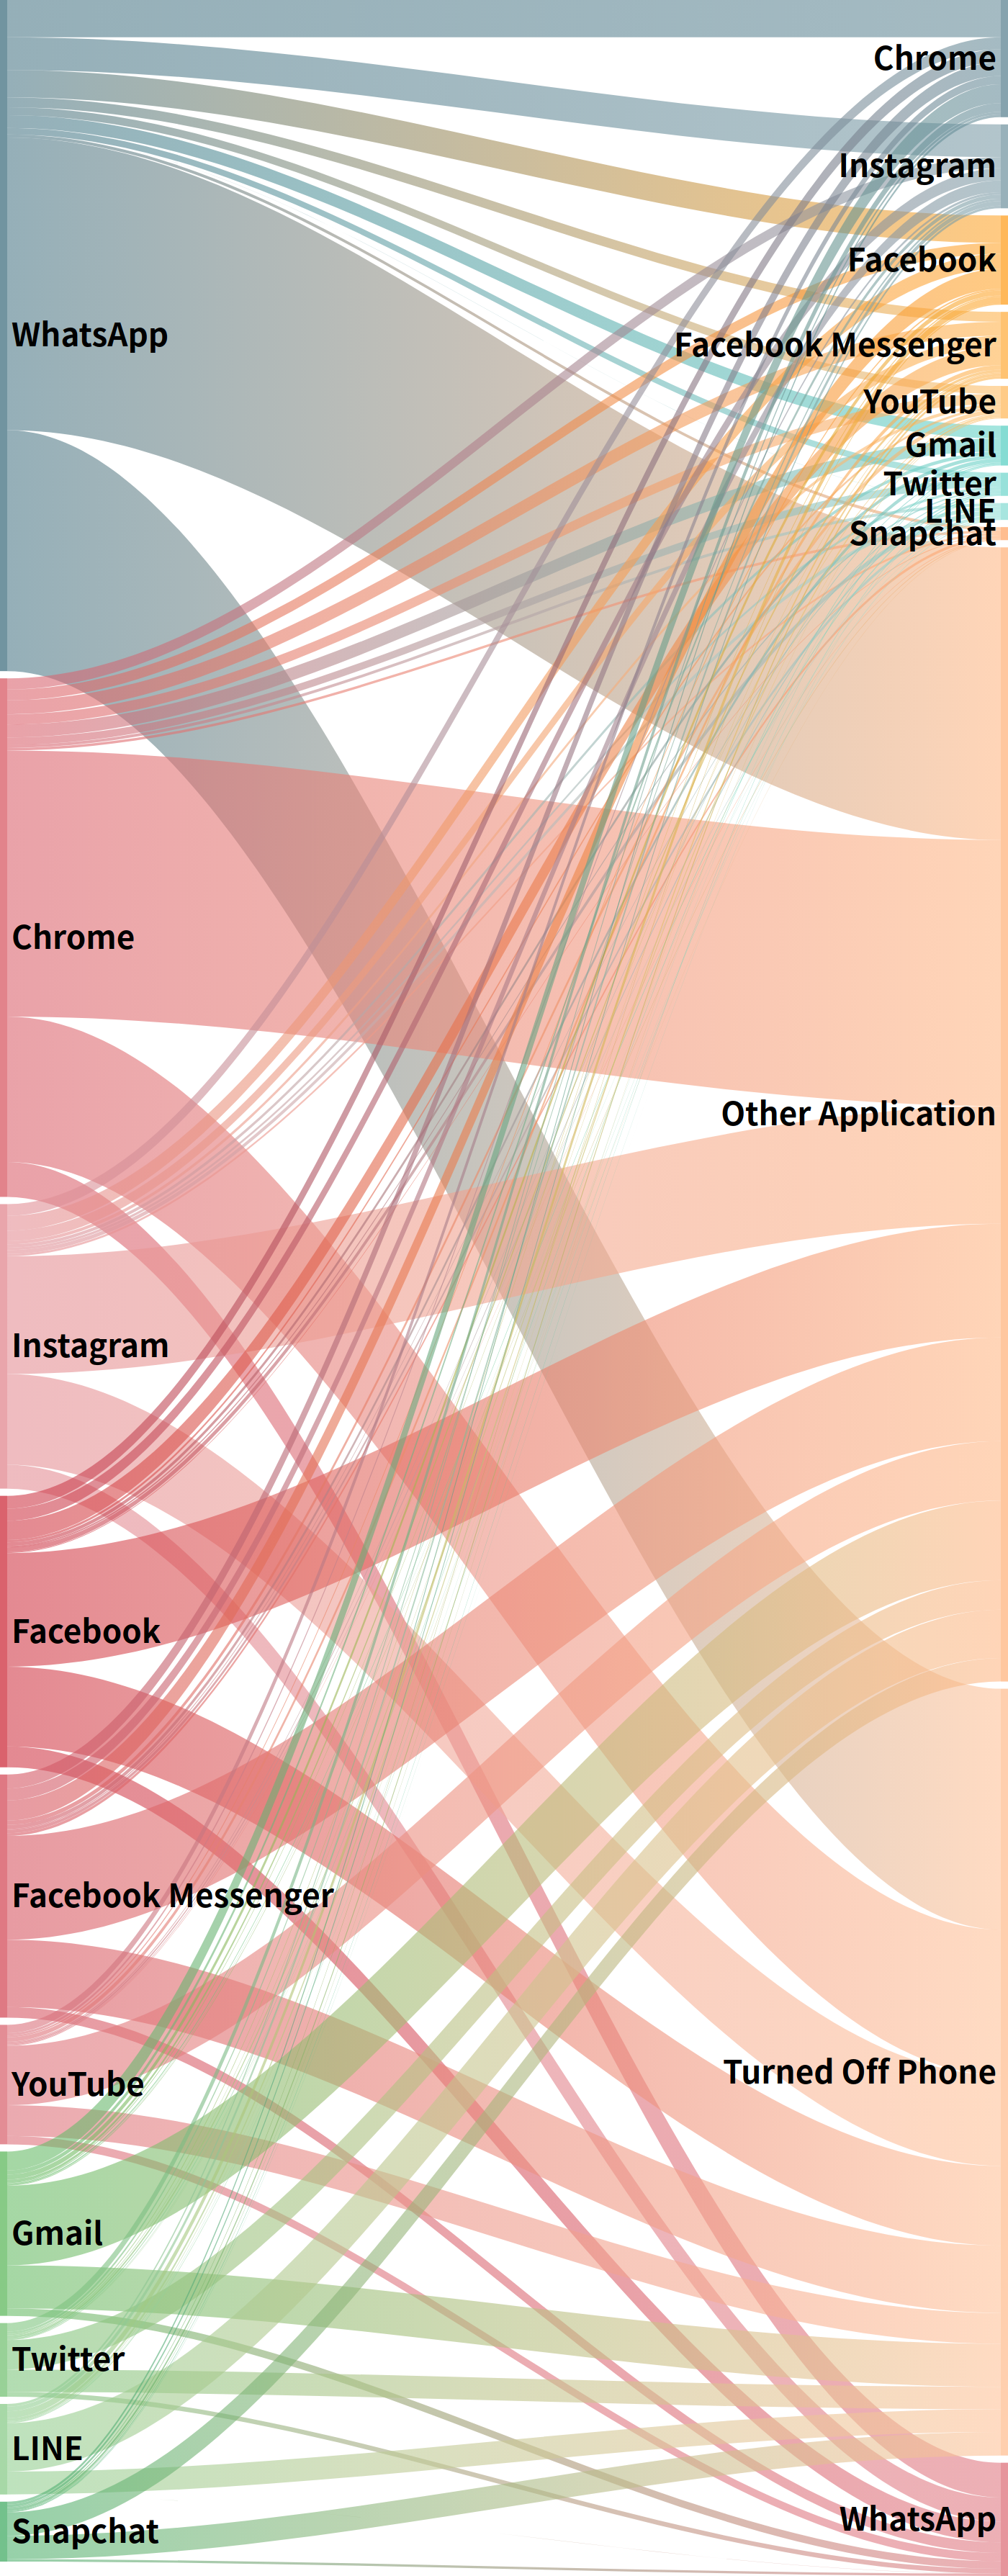
\includegraphics[width=\linewidth]{figures2/android_sankey_v7.png}
\caption{
%\zilin{Maybe the fonts are too small?}
The top 10 goal apps with the most number of sessions on mobile are on the left. On the right is the distribution of where a user ends up immediately after.
%\msb{text is too small to read. Double the font size. Cut some if you need to.  rule of thumb: figure text should never be smaller than the body text of the paper.}
}
  \label{fig:android_sankey_v2} 
\end{figure}

\msb{these figures are going nuts!!! can you fit them on the page?}

\begin{figure}
    \centering
    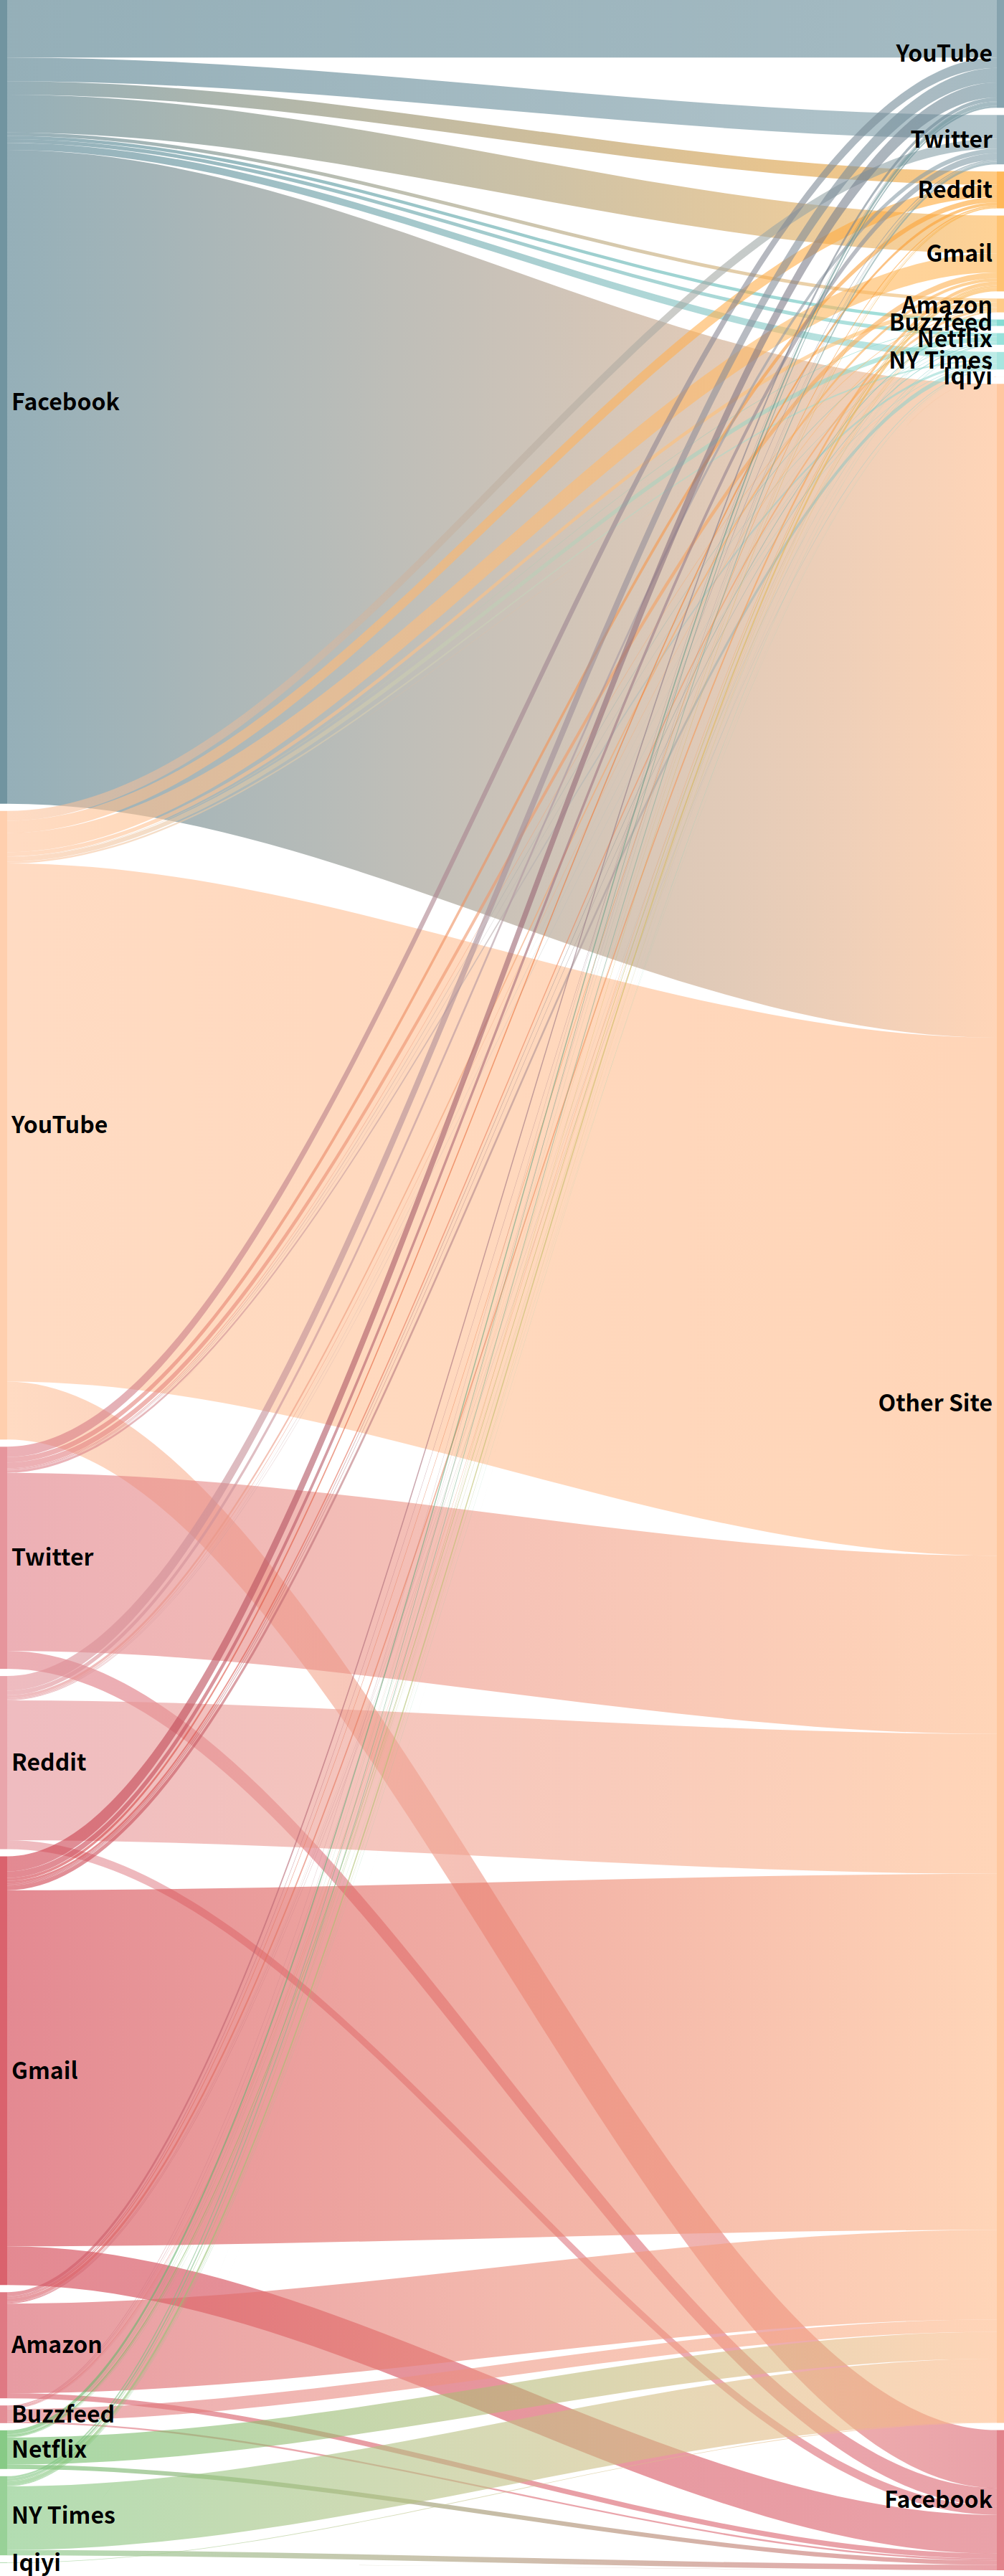
\includegraphics[width=\linewidth]{figures2/browser_sankey_v7.png}
    \caption{The top 10 goal apps with the most number of sessions on the browser are on the left. On the right is the distribution of where a user ends up immediately after.
    %\msb{text is too small to read. Double the font size. Cut some if you need to. rule of thumb: figure text should never be smaller than the body text of the paper.}
    }
    \label{fig:browser_sankey_v2}
\end{figure}



Finally, to build intuition as to the mechanism by which the above effects are happening, we analyzed what happens after users their goal applications. We visualized the flow of sessions from the 10 most widely chosen goal apps and sites in our dataset as Sankey diagrams (Figures~\ref{fig:android_sankey_v2} and \ref{fig:browser_sankey_v2}). On mobile, a majority of sessions end up going to another application, followed by turning off the phone, as shown in Figure~\ref{fig:android_sankey_v2}. On browsers, the majority of sessions went to other sites, as shown in Figure~\ref{fig:browser_sankey_v2}. We can also observe differences in goals users choose on mobile as opposed to desktop -- on mobile, the most popular apps tend to be messaging apps, whereas on the browser they tend to be content aggregators. %These classifications of productivity are taken from crowdsourced user ratings we were able to extract from RescueTime. The majority of sessions end up going to another application, followed by turning off the phone.

%  in Figures~\ref{fig:android_sankey_v2} and \ref{fig:browser_sankey_v2} \msb{this is not the right place to reference the figures; they are results, not method. there should be a point in results where you are looking to these Sankey diagrams to explain what's happening, and the major takeaways from these Sankeys included in the body text}.